\chapter{YOLO}
YOLOs are used for object detection. Other networks also used for objection detection are R-CNN, Fast R-CNN \& Faster R-CNN.

\begin{figure}[h]
  \centering
  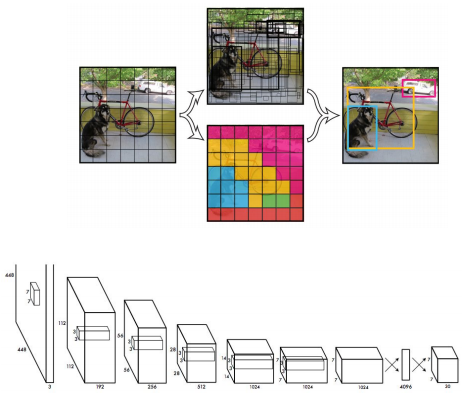
\includegraphics[width=0.5\textwidth]{Images/yolo/1.png}
  \caption{YOLO}
\end{figure}

Another detection strategy that is also commonly used is YOLO. The idea is to solve detection as only a regression problem. Direct prediction using a CNN.

Divide image into $S \times S$ grid, they use $S = 7$. The, within each grid cell predict:
\begin{itemize}
\item $B$ boxes: 4 coordinates + confidence, they use $B = 2$
\item Class scores: $C$ numbers
\end{itemize}

Regression from input image to output $S \times S \times (5*B+C)$ tensor.

It can go at real-time at the expense of lower mAP than Faster R-CNN.